\documentclass[11pt]{article}
\usepackage{mathblatt}


\begin{document}
\pfheftstil
\pfheftkopf{Koerper}{P10}
\pfrueckblick
\begin{pfaufg}{}{1.}{}
Ergänze die Tabelle d | r | r².
\par\smallskip\noindent \begingroup\renewcommand{\arraystretch}{1.3}\begin{tabular}{|c|c|c|}\hline \textbf{d} & \textbf{r} & \textbf{r²} \\ \hline 6 cm | 36 cm² & \rule{0pt}{3ex}\hspace{1.6cm} & \rule{0pt}{3ex}\hspace{1.6cm} \\ \hline 3,2 cm | 10,24 cm² & \rule{0pt}{3ex}\hspace{1.6cm} & \rule{0pt}{3ex}\hspace{1.6cm} \\ \hline 29 cm | 841 cm² & \rule{0pt}{3ex}\hspace{1.6cm} & \rule{0pt}{3ex}\hspace{1.6cm} \\ \hline\end{tabular}\endgroup\par
\fusshilfe{\mbox{1:~6 cm | 36 cm²; 3,2 cm | 10,24 cm²; 29 cm | 841 cm²}}
\end{pfaufg}
\begin{pfaufg}{}{2.}{}
Ergänze die Tabelle Körper | Flächen.
\par\smallskip\noindent \begingroup\renewcommand{\arraystretch}{1.3}\begin{tabular}{|c|c|}\hline \textbf{Körper} & \textbf{Flächen} \\ \hline 2 Dreiecke und 3 Rechtecke & \rule{0pt}{3ex}\hspace{1.6cm} \\ \hline 4 Dreiecke & \rule{0pt}{3ex}\hspace{1.6cm} \\ \hline 2 Kreise und 1 Rechteck & \rule{0pt}{3ex}\hspace{1.6cm} \\ \hline\end{tabular}\endgroup\par
\fusshilfe{\mbox{2:~2 Kreise und 1 Rechteck}}
\end{pfaufg}
\pfstufekopf[svolumendirekt]{Volumen direkt}{in 4 der letzten 5 Prüfungen}
\pfgruppe{}
\begin{pfaufg}{}{3.}{}
Ein Ball passt genau in eine Schachtel. Die Schachtel ist $22$ cm breit. Kreuze an, ob die $22$ cm der Radius oder der Durchmesser des Balls sind.
\pfkreuzzeile{Radius}\pfkreuzzeile{Durchmesser}
\fusshilfe{\mbox{3:~Durchmesser}}
\end{pfaufg}
\begin{pfaufg}{}{4.}{}
Eine Tasse ist oben $8$ cm breit, von Rand zu Rand durch die Mitte gemessen. Ist das der Radius oder der Durchmesser? Gib den Radius an.
\par\noindent Radius \leerfeld[cm] \par
\fusshilfe{\mbox{4:~Radius $4$ cm}}
\end{pfaufg}
\begin{pfaufg}{}{5.}{}
Du willst wissen, wie viel Wasser in ein Aquarium passt. Kreuze an, was du berechnen musst.
\pfkreuzzeile{Volumen}\pfkreuzzeile{Oberfläche}
\fusshilfe{\mbox{5:~Volumen}}
\end{pfaufg}
\begin{pfaufg}{}{6.}{}
Eine Tonne hat den Durchmesser $0{,}5$ m und die Höhe $70$ cm. Schreibe vor dem Rechnen beide Maße in cm.
\par\noindent \leerfeld[cm]  und \leerfeld[cm] \par
\fusshilfe{\mbox{6:~$50$ cm und $70$ cm}}
\end{pfaufg}
\begin{pfaufg}{}{7.}{}
Eine Strecke geht von der Spitze eines Kegels zum Rand des Grundkreises. Kreuze an, wie diese Strecke heißt.
\pfkreuzzeile{Höhe}\pfkreuzzeile{Mantellinie}\pfkreuzzeile{Radius}
\fusshilfe{\mbox{7:~Mantellinie}}
\end{pfaufg}
\begin{pfaufg}{}{8.}{}
Ein Zelt hat die Form des Prismas im Bild. Färbe die Grundfläche. Zeichne die Höhe des Prismas farbig nach.
\par\smallskip\noindent \prismadreieck{4}{2.5}{2}{}{}{}\par
\rechenraster{1}
\fusshilfe{\mbox{8:~auch wenn das Prisma liegt}}
\end{pfaufg}
\begin{pfaufg}{}{9.}{}
Die Figur zeigt das Netz einer Pyramide. Eine Strecke ist mit ? markiert. Kreuze an, wie diese Strecke heißt.
\pfkreuzzeile{Höhe}\pfkreuzzeile{Seitenhöhe}\pfkreuzzeile{Seitenkante}
\par\smallskip\noindent \netzpyramide{2.5}{2}{}{?}\par
\fusshilfe{\mbox{9:~Seitenhöhe}}
\end{pfaufg}
\begin{pfaufg}{}{10.}{}
Die Figur zeigt ein Turmdach in Form einer Pyramide. Zeichne das rechtwinklige Dreieck aus Höhe, halber Grundkante und Seitenhöhe ein. Markiere die Hypotenuse. Du musst nichts rechnen.
\par\smallskip\noindent \pyramide{4}{4}{3}{$6$ m}{}{$4$ m}\par
\rechenraster{1}
\end{pfaufg}
\pfgruppe{}
\begin{pfaufg}{P10 ’26}{11.}{}
Ein Würfel hat die Kantenlänge a = 3 cm. Gib sein Volumen an.
\rechenraster{1}
\fusshilfe{\mbox{11:~27 cm³}}
\end{pfaufg}
\pfgruppe{}
\begin{pfaufg}{SH ’23}{12.}{}
Unter einem Pool muss auf einer Fläche von 6,50 m × 4,50 m die Erde 30 cm tief ausgetauscht werden. Berechne, wie viel m³ Erde das sind.
\rechenraster{1}
\fusshilfe{\mbox{12:~V = 6,5 · 4,5 · 0,3 $\approx$ 8,8 m³}}
\end{pfaufg}
\pfgruppe{}
\begin{pfaufg}{P10 ’14}{13.}{}
Für ein Café wird eine Kühlvitrine in Form eines Prismas gebaut. Die Grundfläche ist ein gleichschenkliges Trapez mit den parallelen Seiten 110 cm und 80 cm, den Schenkeln 57 cm und dem Flächeninhalt 5 225 cm². Die Vitrine ist 165 cm hoch. Berechne das Volumen der Vitrine.
\par\smallskip\noindent \begin{tikzpicture}[line width=0.6pt,baseline=(current bounding box.north)]\draw (-1.50,3.70) -- (1.50,3.70) -- (1.09,2.80) -- (-1.09,2.80) -- cycle;\draw (1.50,0.90) -- (1.09,0.00) -- (-1.09,0.00) -- (-1.50,0.90);\draw[dashed] (-1.50,0.90) -- (1.50,0.90);\draw[dashed] (-1.50,0.90) -- (-1.50,3.70);\draw (1.50,0.90) -- (1.50,3.70);\draw (1.09,0.00) -- (1.09,2.80);\draw (-1.09,0.00) -- (-1.09,2.80);\path (-1.50,3.70) -- node[font=\scriptsize,above] {110} (1.50,3.70);\path (-1.09,0.00) -- node[font=\scriptsize,below] {80} (1.09,0.00);\path (1.09,2.80) -- node[font=\scriptsize,right] {57} (1.50,3.70);\path (1.09,0.00) -- node[font=\scriptsize,right] {165} (1.09,2.80);\node[font=\scriptsize,mbgrau,anchor=north west] at (-2,-0.4) {Maße in cm};\node[font=\scriptsize,mbgrau,anchor=north west] at ([yshift=-2pt]current bounding box.south west) {nicht maßstabsgerecht};\end{tikzpicture}\par
\rechenraster{1}
\fusshilfe{\mbox{13:~862 125 cm³ ($\approx$ 0,86 m³)}}
\end{pfaufg}
\pfgruppe{}
\begin{pfaufg}{P10 ’16}{14.}{}
Eine Kugel zum Kugelstoßen hat einen Durchmesser von 12 cm. Berechne ihr Volumen.
\rechenraster{2}
\fusshilfe{\mbox{14:~288$\pi$ $\approx$ 904,8 cm³}}
\end{pfaufg}
\pfgruppe{}
\begin{pfaufg}{P10 ’22}{15.}{}
Ein Becher hat die Form eines Zylinders ohne Deckel. Er ist h = 7 cm hoch und hat den Radius r = 3,2 cm. Zeige, dass 200 ml Flüssigkeit in den Becher passen (1 cm³ = 1 ml).
\par\smallskip\noindent \begin{tikzpicture}[line width=0.6pt,baseline=(current bounding box.north)]\fill[black!15] (-1.1,0) arc (180:360:1.1 and 0.33) -- (1.1,2.4) arc (0:-180:1.1 and 0.33) -- cycle;\draw (-1.10,0.00) arc (180:360:1.10 and 0.33);\draw[dashed] (1.10,0.00) arc (0:180:1.10 and 0.33);\draw (-1.1,0) -- (-1.1,2.4); \draw (1.1,0) -- (1.1,2.4);\draw (0,2.4) ellipse (1.1 and 0.33);\node[font=\scriptsize,mbgrau,anchor=north west] at ([yshift=-2pt]current bounding box.south west) {nicht maßstabsgerecht};\end{tikzpicture}\par
\rechenraster{2}
\fusshilfe{\mbox{15:~71,68$\pi$ $\approx$ 225,2 cm³ > 200 ml}}
\end{pfaufg}
\pfgruppe{}
\begin{pfaufg}{P10 ’23}{16.}{}
Eine Konservendose hat die Form eines Zylinders mit dem Radius 4 cm und der Höhe 8 cm. Auf der Dose steht: Inhalt etwa 400 ml. Weise nach, dass das stimmt (1 cm³ = 1 ml).
\par\smallskip\noindent \begin{tikzpicture}[line width=0.6pt,baseline=(current bounding box.north)]\draw (-1.10,0.00) arc (180:360:1.10 and 0.33);\draw[dashed] (1.10,0.00) arc (0:180:1.10 and 0.33);\draw (-1.1,0) -- (-1.1,2.4); \draw (1.1,0) -- (1.1,2.4);\draw (0,2.4) ellipse (1.1 and 0.33);\node[font=\scriptsize,mbgrau,anchor=north west] at ([yshift=-2pt]current bounding box.south west) {nicht maßstabsgerecht};\end{tikzpicture}\par
\rechenraster{2}
\fusshilfe{\mbox{16:~wahr, V = $\pi$ · 4² · 8 = 128$\pi$ $\approx$ 402,1 cm³ $\approx$ 400 ml}}
\end{pfaufg}
\pfgruppe{}
\begin{pfaufg}{P10 ’21}{17.}{}
Herr Gärtner stellt eine Regentonne in Form eines Zylinders auf. Sie ist h = 95 cm hoch und hat den Radius r = 29 cm. Der Hersteller gibt an, dass etwa 250 Liter Wasser in die Tonne passen. Bestätige diese Angabe mit einer Rechnung (1 l = 1 dm³).
\par\smallskip\noindent \begin{tikzpicture}[line width=0.6pt,baseline=(current bounding box.north)]\draw (-1.10,0.00) arc (180:360:1.10 and 0.33);\draw[dashed] (1.10,0.00) arc (0:180:1.10 and 0.33);\draw (-1.1,0) -- (-1.1,2.4); \draw (1.1,0) -- (1.1,2.4);\draw (0,2.4) ellipse (1.1 and 0.33);\draw (-1.1,0.7) arc (180:360:1.1 and 0.33);\draw (-1.1,1.7) arc (180:360:1.1 and 0.33);\node[font=\scriptsize,mbgrau,anchor=north west] at ([yshift=-2pt]current bounding box.south west) {nicht maßstabsgerecht};\end{tikzpicture}\par
\rechenraster{2}
\fusshilfe{\mbox{17:~V = $\pi$ · 29² · 95 $\approx$ 250 998 cm³ $\approx$ 251 l}}
\end{pfaufg}
\pfsteckt{steckt auch in Nr. 28 (P10 ’24)}
\pfstufekopf[snetzerkennen]{Netz erkennen}{in 1 der letzten 5 Prüfungen}
\pfgruppe{}
\begin{pfaufg}{nach P10 ’17}{18.}{}
Ein Zelt hat die Form im Bild. Kreuze an, welcher Körper es ist. 
\pfkreuzzeile{Pyramide}\pfkreuzzeile{Prisma}\pfkreuzzeile{Quader}
\par\smallskip\noindent \prismadreieck{4}{2}{2.5}{}{}{}\par
\fusshilfe{\mbox{18:~Prisma}}
\end{pfaufg}
\pfgruppe{}
\begin{pfaufg}{P10 ’17}{19.}{}
Die Abbildung zeigt einen Körper im Schrägbild. Kreuze an, welcher Körper es ist:
\pfkreuzzeile{Pyramide}\pfkreuzzeile{Prisma}\pfkreuzzeile{Quader}
\par\smallskip\noindent 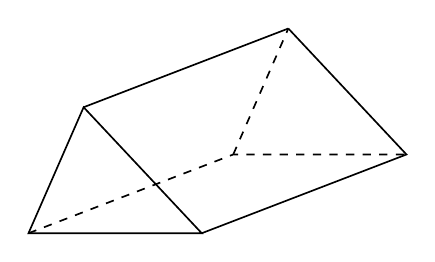
\begin{tikzpicture}[line width=0.6pt,baseline=(current bounding box.north)]\draw (0.00,0.00) -- (2.20,0.00) -- (0.70,1.60) -- cycle;\draw (3.30,2.60) -- (4.80,1.00) -- (2.20,0.00); \draw[dashed] (0.00,0.00) -- (2.60,1.00) -- (4.80,1.00);\draw (0.70,1.60) -- (3.30,2.60); \draw[dashed] (2.60,1.00) -- (3.30,2.60);\end{tikzpicture}\par
\fusshilfe{\mbox{19:~Prisma}}
\end{pfaufg}
\begin{pfaufg}{P10 ’18}{20.}{}
Kreuze an, welcher Körper zu dem abgebildeten Netz gehört:
\pfkreuzzeile{Prisma}\pfkreuzzeile{Pyramide}\pfkreuzzeile{Quader}
\par\smallskip\noindent 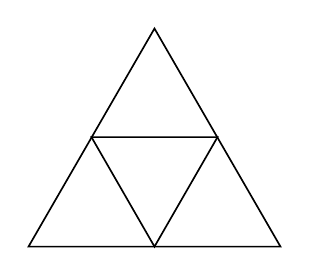
\begin{tikzpicture}[line width=0.6pt,baseline=(current bounding box.north)]\draw (0.00,0.00) -- (3.20,0.00) -- (1.60,2.77) -- cycle;\draw (1.60,0.00) -- (2.40,1.39) -- (0.80,1.39) -- cycle;\end{tikzpicture}\par
\fusshilfe{\mbox{20:~Pyramide}}
\end{pfaufg}
\pfgruppe{}
\begin{pfaufg}{P10 ’16}{21.}{}
Aus dem abgebildeten Netz wird ein Würfel gefaltet. Nach dem Falten liegt die graue Fläche oben. Markiere die Fläche, die dann unten liegt.
\par\smallskip\noindent 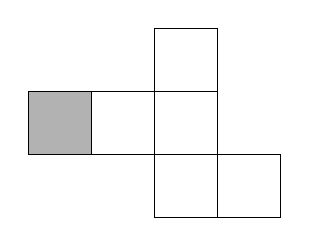
\begin{tikzpicture}[line width=0.6pt,baseline=(current bounding box.north)]\draw (1.60,1.60) rectangle ++(0.8,0.8);\draw (1.60,0.80) rectangle ++(0.8,0.8);\draw (1.60,0.00) rectangle ++(0.8,0.8);\draw (0.80,0.80) rectangle ++(0.8,0.8);\draw[fill=black!30] (0.00,0.80) rectangle ++(0.8,0.8);\draw (2.40,0.00) rectangle ++(0.8,0.8);\end{tikzpicture}\par
\rechenraster{1}
\fusshilfe{\mbox{21:~mittleres Quadrat der senkrechten Dreierreihe}}
\end{pfaufg}
\pfgruppe{}
\begin{pfaufg}{P10 ’22}{22.}{}
Ein Becher hat die Form eines Zylinders ohne Deckel. Er ist h = 7 cm hoch und hat den Radius r = 3,2 cm. Kreuze an, welches der drei Netze zum Becher passt. Ermittle die Länge und die Breite der Mantelfläche.
\par\smallskip\noindent 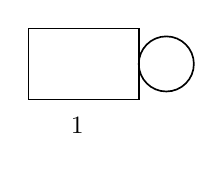
\begin{tikzpicture}[line width=0.6pt,baseline=0]\draw (0,0) rectangle (1.40,0.90); \draw (1.75,0.45) circle (0.35);\node[font=\small,anchor=north] at (0.70,-0.1) {1\enspace$\square$};\end{tikzpicture}\hspace{0.7cm}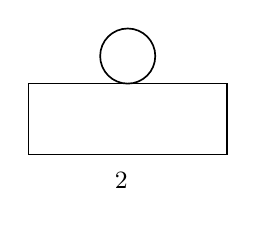
\begin{tikzpicture}[line width=0.6pt,baseline=0]\draw (0,0) rectangle (2.52,0.90); \draw (1.26,1.25) circle (0.35);\node[font=\small,anchor=north] at (1.26,-0.1) {2\enspace$\square$};\end{tikzpicture}\hspace{0.7cm}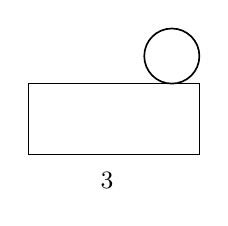
\begin{tikzpicture}[line width=0.6pt,baseline=0]\draw (0,0) rectangle (2.17,0.90); \draw (1.82,1.25) circle (0.35);\node[font=\small,anchor=north] at (1.08,-0.1) {3\enspace$\square$};\end{tikzpicture}\par
\pfzwfrage{Gib an, welcher Länge des Bechers die lange Seite der Mantelfläche entspricht.}
\rechenraster{2}
\fusshilfe{\mbox{22:~drittes Netz; Länge 6,4$\pi$ $\approx$ 20,1 cm, Breite 7 cm}}
\end{pfaufg}
\pfstufekopf[srckwrtsradiusoderhhe]{rückwärts: Radius oder Höhe aus Volumen}{in 2 der letzten 5 Prüfungen}
\pfgruppe{}
\begin{pfaufg}{nach P10 ’22}{\llap{\textasteriskcentered\,}23.}{}
Ein Eimer soll bei $15$ cm Höhe $2\,000$ cm³ fassen. Berechne den Radius. Runde auf eine Stelle nach dem Komma.
\par\noindent \leerfeld[cm] \par
\fusshilfe{\mbox{23:~$\approx 6{,}5$ cm}}
\end{pfaufg}
\pfgruppe{}
\begin{pfaufg}{P10 ’23}{\llap{\textasteriskcentered\,}24.}{}
Eine Konservendose hat die Form eines Zylinders mit dem Radius 4 cm und der Höhe 8 cm. Mit denselben Deckeln (r = 4 cm) soll auch eine größere Dose mit 1 Liter Inhalt gebaut werden. Ermittle ihre Höhe.
\par\smallskip\noindent \begin{tikzpicture}[line width=0.6pt,baseline=(current bounding box.north)]\draw (-1.10,0.00) arc (180:360:1.10 and 0.33);\draw[dashed] (1.10,0.00) arc (0:180:1.10 and 0.33);\draw (-1.1,0) -- (-1.1,2.4); \draw (1.1,0) -- (1.1,2.4);\draw (0,2.4) ellipse (1.1 and 0.33);\node[font=\scriptsize,mbgrau,anchor=north west] at ([yshift=-2pt]current bounding box.south west) {nicht maßstabsgerecht};\end{tikzpicture}\par
\pfzwfrage{Rechne 1 Liter in cm³ um.}
\pfzwfrage{Berechne die Grundfläche der Dose.}
\rechenraster{2}
\fusshilfe{\mbox{24:~h = 125/(2$\pi$) $\approx$ 19,9 cm}}
\end{pfaufg}
\pfgruppe{}
\begin{pfaufg}{P10 ’22}{\llap{\textasteriskcentered\,}25.}{}
Ein Becher hat die Form eines Zylinders ohne Deckel. Er ist h = 7 cm hoch und hat den Radius r = 3,2 cm. Ein größerer Becher soll 425 ml fassen und wieder 7 cm hoch sein. Berechne seinen Radius.
\par\smallskip\noindent \begin{tikzpicture}[line width=0.6pt,baseline=(current bounding box.north)]\fill[black!15] (-1.1,0) arc (180:360:1.1 and 0.33) -- (1.1,2.4) arc (0:-180:1.1 and 0.33) -- cycle;\draw (-1.10,0.00) arc (180:360:1.10 and 0.33);\draw[dashed] (1.10,0.00) arc (0:180:1.10 and 0.33);\draw (-1.1,0) -- (-1.1,2.4); \draw (1.1,0) -- (1.1,2.4);\draw (0,2.4) ellipse (1.1 and 0.33);\node[font=\scriptsize,mbgrau,anchor=north west] at ([yshift=-2pt]current bounding box.south west) {nicht maßstabsgerecht};\end{tikzpicture}\par
\pfzwfrage{Stelle die Volumenformel mit den gegebenen Werten auf.}
\rechenraster{3}
\fusshilfe{\mbox{25:~r = √(425/(7$\pi$)) $\approx$ 4,40 cm}}
\end{pfaufg}
\pfstufekopf[srestvolumen]{Restvolumen}{in 1 der letzten 5 Prüfungen}
\pfgruppe{}
\begin{pfaufg}{}{26.}{}
Ein Haus hat ein Satteldach. Aus welchen zwei Körpern besteht das Haus?
\rechenraster{1}
\fusshilfe{\mbox{26:~Quader und Dreiecksprisma}}
\end{pfaufg}
\pfgruppe{}
\begin{pfaufg}{NI ’23}{27.}{}
Ein kugelförmiger Gasspeicher hat außen 27 m Durchmesser. Seine Metallwand ist 0,03 m dick. Berechne das Volumen innen.
\rechenraster{2}
\fusshilfe{\mbox{27:~13,47 m; $\approx$ 10 237,44 m³}}
\end{pfaufg}
\pfgruppe{}
\begin{pfaufg}{P10 ’24}{\llap{\textasteriskcentered\,}28.}{}
Eine Firma stellt Kegel mit dem Radius r = 30 cm und der Höhe h = 80 cm her. Eine andere Firma verschickt denselben Kegel in einer zylinderförmigen Verpackung; innen ist sie 81 cm hoch und hat den Radius 30,5 cm. Der freie Raum wird mit Füllmaterial ausgefüllt. Ermittle, wie viele cm³ Füllmaterial man braucht.
\par\smallskip\noindent \begin{tikzpicture}[line width=0.6pt,baseline=(current bounding box.north)]\fill[black!15] (0,0) ellipse (1.2 and 0.36);\draw (-1.20,0.00) arc (180:360:1.20 and 0.36);\draw[dashed] (1.20,0.00) arc (0:180:1.20 and 0.36);\draw (-1.2,0) -- (0,2.4) -- (1.2,0);\node[font=\scriptsize,mbgrau,anchor=north west] at ([yshift=-2pt]current bounding box.south west) {nicht maßstabsgerecht};\end{tikzpicture}\par
\pfzwfrage{Berechne das Volumen der Verpackung.}
\pfzwfrage{Berechne das Volumen des Kegels.}
\rechenraster{3}
\fusshilfe{\mbox{28:~51 350,25$\pi$ $\approx$ 161 322 cm³}}
\end{pfaufg}
\pfstufekopf[smantelflchemitkosten]{Mantelfläche mit Kosten}{in 1 der letzten 5 Prüfungen}
\pfgruppe{}
\begin{pfaufg}{NI ’23}{29.}{}
Eine quadratische Pyramide hat die Grundkante 7 cm und die Seitenhöhe 8,73 cm. Berechne ihre Mantelfläche.
\rechenraster{1}
\fusshilfe{\mbox{29:~M = 4 · ½ · 7 · 8,73 cm² = 122,22 cm²}}
\end{pfaufg}
\pfgruppe{}
\begin{pfaufg}{P10 ’18}{30.}{}
Ein runder Turm hat 6,4 m Durchmesser. Seine zylinderförmige Außenmauer ist 21,7 m hoch und soll renoviert werden. Berechne die Fläche der Außenmauer.
\rechenraster{2}
\fusshilfe{\mbox{30:~138,88$\pi$ $\approx$ 436,3 m²}}
\end{pfaufg}

\par\Needspace*{0.55\textheight}\pfstufekopf[serkennen1]{Was ist gesucht?}{}
\begin{pfaufg}{}{31.}{}
Was ist gesucht? Kreuze an. Rechne nicht.
\par\smallskip\noindent \begingroup\renewcommand{\arraystretch}{1.4}\begin{tabular}{|>{\raggedright\arraybackslash}p{8.3cm}|>{\centering\arraybackslash\hyphenpenalty=0}p{1.55cm}|>{\centering\arraybackslash\hyphenpenalty=0}p{1.55cm}|}\hline  & {\scriptsize\hspace{0pt}Mantelfläche mit Kosten} & {\scriptsize\hspace{0pt}Volumen direkt} \\ \hline Reicht ein Karton von 11 cm × 15 cm für die Mäntel von Hut und Rumpf der Puppe? & $\square$ & $\square$ \\ \hline Ein Würfel hat die Kantenlänge 3 cm. Wie groß ist sein Rauminhalt? & $\square$ & $\square$ \\ \hline Die Außenmauer eines runden Turms (d = 6,4 m, 21,7 m hoch) wird gestrichen. Wie groß ist die Fläche? & $\square$ & $\square$ \\ \hline Eine Dose hat den Radius 4 cm und ist 8 cm hoch. Passen 400 ml hinein? & $\square$ & $\square$ \\ \hline Ein Kegeldach (r = 4,7 m, s = 8,6 m) wird mit Ziegeln gedeckt, 1 m² kostet 20 €. Was kosten die Ziegel? & $\square$ & $\square$ \\ \hline Ein Becher ist 7 cm hoch und hat den Radius 3,2 cm. Passen 200 ml hinein? & $\square$ & $\square$ \\ \hline\end{tabular}\endgroup\par
\end{pfaufg}
\pfstufekopf[svergleichenundurteil]{vergleichen und urteilen}{in 1 der letzten 5 Prüfungen}
\pfgruppe{}
\begin{pfaufg}{NI ’24}{32.}{}
Ein Aquarium fasst 300 000 cm³. Ein Fisch braucht 5 000 cm³ Wasser. Paula will 60 Fische einsetzen. Prüfe, ob es groß genug ist.
\rechenraster{1}
\fusshilfe{\mbox{32:~60; es passt genau für 60 Fische}}
\end{pfaufg}
\pfgruppe{}
\begin{pfaufg}{P10 ’21}{\llap{\textasteriskcentered\,}33.}{}
Herr Gärtner stellt eine Regentonne in Form eines Zylinders auf. Sie ist h = 95 cm hoch und hat den Radius r = 29 cm. Herr Gärtner meint: „Eine Tonne mit doppeltem Radius würde genau doppelt so viel Wasser fassen.“ Entscheide, ob das stimmt. Begründe deine Entscheidung.
\par\smallskip\noindent \begin{tikzpicture}[line width=0.6pt,baseline=(current bounding box.north)]\draw (-1.10,0.00) arc (180:360:1.10 and 0.33);\draw[dashed] (1.10,0.00) arc (0:180:1.10 and 0.33);\draw (-1.1,0) -- (-1.1,2.4); \draw (1.1,0) -- (1.1,2.4);\draw (0,2.4) ellipse (1.1 and 0.33);\draw (-1.1,0.7) arc (180:360:1.1 and 0.33);\draw (-1.1,1.7) arc (180:360:1.1 and 0.33);\node[font=\scriptsize,mbgrau,anchor=north west] at ([yshift=-2pt]current bounding box.south west) {nicht maßstabsgerecht};\end{tikzpicture}\par
\rechenraster{1}
\fusshilfe{\mbox{33:~$\approx$ 1004 l)}}
\end{pfaufg}
\pfstufekopf[snetzmitmaenskizziere]{Netz mit Maßen skizzieren}{in 2 der letzten 5 Prüfungen}
\pfgruppe{}
\begin{pfaufg}{P10 ’20}{34.}{}
Eine Schachtel hat die Form eines Prismas. Ihre Grundfläche ist ein Rechteck, 14 cm breit und 12 cm tief. Die vordere Kante ist 6 cm hoch, die hintere 15 cm; die Deckfläche verläuft schräg und ist etwa 16 cm breit. Die beiden Seitenflächen sind Trapeze mit zwei rechten Winkeln. Ein Netz ist schon begonnen. Vervollständige das Netz.
\par\smallskip\noindent \begin{tikzpicture}[line width=0.6pt,baseline=(current bounding box.north)]\draw (0,0) -- (2.8,0) -- (2.8,1.2) -- (0,1.2) -- cycle;\draw (2.8,0) -- (3.6,0.5) -- (3.6,3.5) -- (2.8,1.2);\draw (0,1.2) -- (0.8,3.5) -- (3.6,3.5);\draw[dashed] (0,0) -- (0.8,0.5) -- (3.6,0.5); \draw[dashed] (0.8,0.5) -- (0.8,3.5);\path (0.00,0.00) -- node[font=\scriptsize,below] {14 cm} (2.80,0.00);\path (2.80,0.00) -- node[font=\scriptsize,below right] {12 cm} (3.60,0.50);\path (0.00,0.00) -- node[font=\scriptsize,left] {6 cm} (0.00,1.20);\path (3.60,0.50) -- node[font=\scriptsize,right] {15 cm} (3.60,3.50);\path (0.00,1.20) -- node[font=\scriptsize,left] {16 cm} (0.80,3.50);\draw[mbgitter,line width=0.3pt,step=0.25] (5,-0.5) grid (10.5,3.25);\draw (5.250,0) rectangle ++(2.075,1.500);\draw (7.325,0) rectangle ++(0.750,1.500);\draw (8.075,0) rectangle ++(1.750,1.500);\draw (8.075,1.500) -- (8.075,2.250) -- (9.825,3.375) -- (9.825,1.500);\node[font=\scriptsize,mbgrau,anchor=north west] at (5,-0.5) {1 Kästchen = 2 cm};\node[font=\scriptsize,mbgrau,anchor=north west] at ([yshift=-2pt]current bounding box.south west) {nicht maßstabsgerecht};\end{tikzpicture}\par
\rechenraster{1}
\end{pfaufg}
\pfgruppe{}
\begin{pfaufg}{P10 ’19}{35.}{}
Auf einem Mast sitzt ein dreiseitiges Prisma. Seine drei Seitenflächen sind Rechtecke mit 1,50 m Breite und 1,20 m Höhe; Grund- und Deckfläche sind gleichseitige Dreiecke. Das Netz des Prismas ist schon begonnen. Vervollständige das Netz. Gib die Länge a an.
\par\smallskip\noindent \begin{tikzpicture}[x=0.4cm,y=0.4cm,line width=0.6pt,baseline=(current bounding box.north)]\draw[mbgitter,line width=0.3pt,step=1] (0,0) grid (26,12);\draw (2,7) rectangle ++(5,4); \draw (7,7) rectangle ++(5,4);\draw (7,7) -- (12,7) -- (9.50,2.67) -- cycle;\node[font=\small,anchor=west] at (11.00,4.83) {$a$};\end{tikzpicture}\par
\rechenraster{1}
\fusshilfe{\mbox{35:~a = 1,50 m}}
\end{pfaufg}
\begin{pfaufg}{P10 ’14}{36.}{}
Für ein Café wird eine Kühlvitrine in Form eines Prismas gebaut. Die Grundfläche ist ein gleichschenkliges Trapez mit den parallelen Seiten 110 cm und 80 cm, den Schenkeln 57 cm und dem Flächeninhalt 5 225 cm². Die Vitrine ist 165 cm hoch. Ein Netz der Vitrine ist schon begonnen. Vervollständige das Netz. Gib die fehlenden Maße a, b und d an.
\par\smallskip\noindent 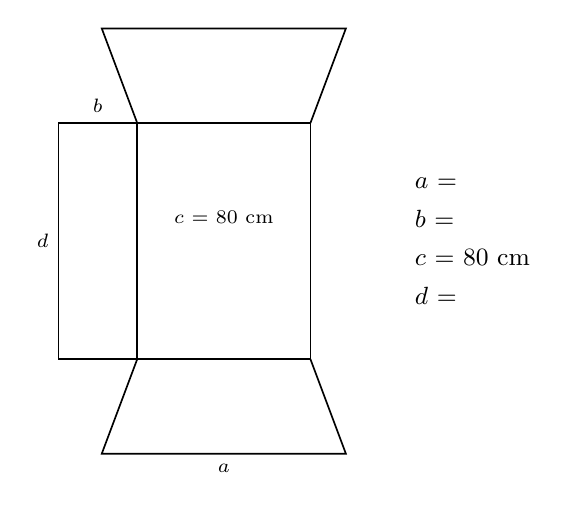
\begin{tikzpicture}[line width=0.6pt,baseline=(current bounding box.north)]\draw (0,0) rectangle (1.0,3.0); \draw (1.0,0) rectangle (3.2,3.0);\draw (1.0,3.0) -- (0.55,4.2) -- (3.6500000000000004,4.2) -- (3.2,3.0);\draw (1.0,0) -- (0.55,-1.2) -- (3.6500000000000004,-1.2) -- (3.2,0);\node[font=\scriptsize,below] at (2.1,-1.2) {$a$};\node[font=\scriptsize,above] at (0.5,3.0) {$b$};\node[font=\scriptsize] at (2.1,1.8) {$c$ = 80 cm};\node[font=\scriptsize,left] at (0,1.5) {$d$};\node[font=\small,anchor=west,align=left] at (4.4,1.5) {$a$ = \leerzelle\\[3pt] $b$ = \leerzelle\\[3pt] $c$ = 80 cm\\[3pt] $d$ = \leerzelle};\end{tikzpicture}\par
\fusshilfe{\mbox{36:~165 cm}}
\end{pfaufg}
\pfgruppe{}
\begin{pfaufg}{P10 ’23}{37.}{}
Eine Konservendose hat die Form eines Zylinders mit dem Radius 4 cm und der Höhe 8 cm. Skizziere die Mantelfläche der Dose. Bestimme ihre Länge a und ihre Breite b und schreibe beide an deine Skizze.
\par\smallskip\noindent \begin{tikzpicture}[line width=0.6pt,baseline=(current bounding box.north)]\draw (-1.10,0.00) arc (180:360:1.10 and 0.33);\draw[dashed] (1.10,0.00) arc (0:180:1.10 and 0.33);\draw (-1.1,0) -- (-1.1,2.4); \draw (1.1,0) -- (1.1,2.4);\draw (0,2.4) ellipse (1.1 and 0.33);\node[font=\scriptsize,mbgrau,anchor=north west] at ([yshift=-2pt]current bounding box.south west) {nicht maßstabsgerecht};\end{tikzpicture}\par
\rechenraster{2}
\fusshilfe{\mbox{37:~Rechteck, a = 8$\pi$ $\approx$ 25,1 cm, b = 8 cm}}
\end{pfaufg}
\pfsteckt{steckt auch in Nr. 22 (P10 ’22)}
\pfstufekopf[skrperimschrgbildskiz]{Körper im Schrägbild skizzieren}{in 1 der letzten 5 Prüfungen}
\pfgruppe{}
\begin{pfaufg}{P10 ’24}{38.}{}
Eine Firma stellt Kegel mit dem Radius r = 30 cm und der Höhe h = 80 cm her. Der Kegel soll in einem quaderförmigen Karton verschickt werden, der möglichst klein ist, in den der Kegel aber ganz hineinpasst. Skizziere den Kegel in den Karton. Kreuze die kleinste passende Größe an (Länge × Breite × Höhe):
\pfkreuzzeile{31 cm × 31 cm × 81 cm}\pfkreuzzeile{61 cm × 61 cm × 101 cm}\pfkreuzzeile{61 cm × 61 cm × 81 cm}\pfkreuzzeile{31 cm × 61 cm × 81 cm. Begründe deine Wahl}
\par\smallskip\noindent 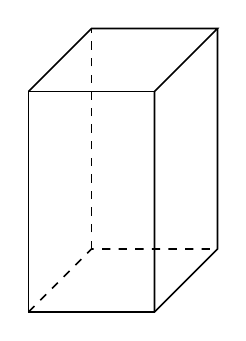
\begin{tikzpicture}[line width=0.6pt,baseline=(current bounding box.north)]\draw (0,0) rectangle (1.6,2.8); \draw (0,2.8) -- (0.8,3.5999999999999996) -- (2.4000000000000004,3.5999999999999996) -- (1.6,2.8) -- (1.6,0);\draw (2.4000000000000004,3.5999999999999996) -- (2.4000000000000004,0.8) -- (1.6,0);\draw[dashed] (0,0) -- (0.8,0.8) -- (2.4000000000000004,0.8); \draw[dashed] (0.8,0.8) -- (0.8,3.5999999999999996);\end{tikzpicture}\par
\rechenraster{1}
\fusshilfe{\mbox{38:~61 cm × 61 cm × 81 cm}}
\end{pfaufg}
\pfgruppe{}
\begin{pfaufg}{P10 ’15}{39.}{}
Mia hat ein Modell einer Pyramide mit quadratischer Grundfläche gebaut: Es ist 0,68 m hoch, die Grundkante ist 0,80 m lang. Zeichne in das Schrägbild die Höhe der Pyramide ein. Beschrifte die Skizze mit den gegebenen Maßen.
\par\smallskip\noindent \begin{tikzpicture}[line width=0.6pt,baseline=(current bounding box.north)]\draw (0,0) -- (2.4,0) -- (3.3,0.9);\draw[dashed] (3.3,0.9) -- (0.9,0.9) -- (0,0); \draw[dashed] (0.9,0.9) -- (1.65,2.6);\draw (0,0) -- (1.65,2.6);\draw (2.4,0) -- (1.65,2.6);\draw (3.3,0.9) -- (1.65,2.6);\node[font=\scriptsize,mbgrau,anchor=north west] at ([yshift=-2pt]current bounding box.south west) {nicht maßstabsgerecht};\end{tikzpicture}\par
\rechenraster{1}
\fusshilfe{\mbox{39:~0,68 m; Grundkante 0,80 m}}
\end{pfaufg}
\pfpruefstein{P10 ’26}
\begin{pfaufg}{}{}{}
Ein Turm besteht unten aus einem Zylinder, sein Dach ist ein Kegel. Bekannt sind: h = 25,0 m (Höhe des Zylinders), r = 4,7 m (Radius von Zylinder und Kegel) und s = 8,6 m (Mantellinie des Kegels).
\par\smallskip\noindent \begin{tikzpicture}[line width=0.6pt,baseline=(current bounding box.north)]\draw (-1.00,0.00) arc (180:360:1.00 and 0.30);\draw[dashed] (1.00,0.00) arc (0:180:1.00 and 0.30);\draw (-1.0,0) -- (-1.0,2.6); \draw (1.0,0) -- (1.0,2.6);\draw (-1.00,2.60) arc (180:360:1.00 and 0.30);\draw[dashed] (1.00,2.60) arc (0:180:1.00 and 0.30);\draw (-1.0,2.6) -- (0,3.9000000000000004) -- (1.0,2.6);\draw[dashed] (0,2.6) -- (1.0,2.6);\node[font=\scriptsize,right] at (1.0,1.3) {$h$ = 25,0 m};\node[font=\scriptsize,below,fill=white,inner sep=1pt] at (0.5,2.52) {$r$ = 4,7 m};\node[font=\scriptsize,right] at (0.55,3.35) {$s$ = 8,6 m};\node[font=\scriptsize,mbgrau,anchor=north west] at ([yshift=-2pt]current bounding box.south west) {nicht maßstabsgerecht};\end{tikzpicture}\par
\end{pfaufg}
\begin{pfaufg}{}{a)}{2 BE}
Berechne das Volumen des zylinderförmigen Teils.
\rechenplatz{3}
\fusshilfe{\mbox{Prüfstein a):~552,25$\pi$ $\approx$ 1734,9 m³}}
\end{pfaufg}
\begin{pfaufg}{}{b)}{3 BE}
Das Dach wird mit Ziegeln gedeckt; 1 m² Ziegel kostet 20,00 €. Berechne die Kosten für die Ziegel.
\rechenplatz{3}
\fusshilfe{\mbox{Prüfstein b):~$\approx$ 2539,66 € (rund 2540 €)}}
\end{pfaufg}
\begin{pfaufg}{}{*c)}{3 BE}
Ein Turm besteht aus einem Zylinder (Höhe 25,0 m, Radius 4,7 m) mit einem Kegeldach; die Mantellinie des Kegels ist 8,6 m lang, sein Radius ebenfalls 4,7 m. Bestimme die Gesamthöhe des Turms.
\rechenplatz{3}
\fusshilfe{\mbox{Prüfstein c):~25 + √51,87 $\approx$ 32,2 m}}
\end{pfaufg}
\begin{pfaufg}{}{*d)}{3 BE}
Ein Zylinder und ein Kegel sind gleich hoch. Jemand behauptet: „Ist der Radius des Kegels dreimal so groß wie der des Zylinders, haben beide dasselbe Volumen.“ Untersuche mit einer Rechnung, ob das stimmt.
\rechenplatz{3}
\fusshilfe{\mbox{Prüfstein d):~3 · V\_Zylinder $\Rightarrow$ dreifaches Volumen}}
\end{pfaufg}
\end{document}